%%% Laboratory	 Notes
%%% Template by Mikhail Klassen, April 2013
%%% Contributions from Sarah Mount, May 2014
\documentclass[a4paper]{tufte-handout}

\newcommand{\workingDate}{\textsc{Fall $|$ 2016}}
\newcommand{\userName}{Cail Daley}
\newcommand{\institution}{Wesleyan University}

\usepackage{aumic_notes}


\usepackage{hyperref}
\usepackage{hypcap}
\hypersetup{
    pdffitwindow=false,            % window fit to page
    pdfstartview={Fit},            % fits width of page to window
    pdftitle={HD_100546_Modeling_Notes},     % document title
    pdfauthor={Cail Daley},         % author name
    pdfsubject={},                 % document topic(s)
    pdfnewwindow=true,             % links in new window
    colorlinks=true,               % coloured links, not boxed
    linkcolor=DarkScarletRed,      % colour of internal links
    citecolor=DarkChameleon,       % colour of links to bibliography
    filecolor=DarkPlum,            % colour of file links
    urlcolor=DarkSkyBlue           % colour of external links
}

\title{AU Mic Notes}
\date{2016}

\begin{document}
\maketitle

%%%%%%%%%%%%%%%%%%%%%%%%%%%%%%%%%%%%%%%%%%%%%%%%%%%%%%%%

\begin{tasks}
	\begin{itemize}
		\item Write up :/
	\end{itemize}
\end{tasks}

%%%%%%%%%%%%%%%%%%%%%%%%%%%%%%%%%%%%%%%%%%%%%%%%%%%%%%%%

\begin{maybe}
	\begin{itemize}
		\item
	\end{itemize}
\end{maybe}

%%%%%%%%%%%%%%%%%%%%%%%%%%%%%%%%%%%%%%%%%%%%%%%%%%%%%%%%

\begin{mer}
	\begin{itemize}
		\item
	\end{itemize}

\end{mer}
%%%%%%%%%%%%%%%%%%%%%%%%%%%%%%%%%%%%%%%%%%%%%%%%%%%%%%%%

\newday{13 January 2017}
AU Mic was observed on three dates with ALMA: 26 March 2014, 18 August 2014, and 24 June 2015. All observations were configured with four spectral windows, and used 12 m antennas with ALMA's Band 7 receivers. One spectral window was centered around the CO $J = (2-1)$ transition at a frequency of 230.538001 Ghz, while the other three were configured to detect continuum with maximum bandwidth of 2 Ghz and channel spacing of 15.6 Mhz. Central frequencies for spectral windows 1-3 can be found in Table 1.

The 26 March data were obtained with 32 antennas and baselines ranging between  14 and 437 m; weather conditions were excellent ($\sim$0.6 mm of precipitable water vapor). The quasar J1924-2914 was used as a bandpass calibrator, and Titan was used to calibrate absolute flux. After these initial calibrations, observations cycled every seven minutes between AU Mic and the quasar J2101-2933, which was used for phase calibration. In total, 35 minutes were spent on source.

The 18 August utilized 35 antennas in a more extended antenna configuration (baselines between 20 and 1268 m) to probe the small scale structure of the disk. Weather conditions were poorer, with $\sim$1.6 mm of precipitable water vapor. The quasars J2056-4714 and J2056-472 were used as bandpass and absolute flux calibrators respectively, and were observed at the beginning of the observation window. For the remainder of the time block, antennas cycled between seven-minute observations of AU Mic and brief observations of the quasars J2101-2933 (phase calibration) and J2057-3734 (delay calibration). AU Mic was observed for 35 minutes altogether.

The 24 June observation was taken to supplement the 18 August's, which was of poor quality due to ? (I don't remember why...). 37 antennas covered baselines from 30 to 1431 m and weather condition were good-- 0.7 mm of precipitable water vapor. Bandpass and absolute flux calibrations, using J1924-2914 and Titan respectively, were conducted at the beginning of the scheduled time block. Short observations of the phase calibrator J2056-3208 and the delay calibrator J2101-2933 were interspersed among seven-minute observations of the source, which was observed for 33 minutes.

Calibration, reduction, and imaging were carried out using the CASA and MIRIAD software packages.

\begin{itemize}
	\item 18 aug
	      \begin{itemize}
	      	\item PWV roughly 1.6mm
	      	\item Objects:
	      	      \begin{itemize}
	      	      	\item AU Mic: around 6m per observation, 5 observations
	      	      	\item J2056-4714: bandpass calibrator, observed for \abt 5 min at beginning
	      	      	\item J2056-472: amplitude calibrator, observed for \abt 3 min at beginning
	      	      	\item J2101-2933: phase calibrator, observed for \abt 1 m each, 4 times
	      	      	\item J2057-3734: delay calibrator, observed for \abt 1 m each, 4 times
	      	      \end{itemize}
	      	\item spws:
	      	      \begin{itemize}
	      	      	\item 0: ctr=230538 Mhz, totBW=1875000 khz, chanwid=488 kHz
	      	      	\item 1: ctr=228492 Mhz, totBW=2e6 khz, chanwid=15625 khz
	      	      	\item 1: ctr=213492 Mhz, totBW=2e6 khz, chanwid=-15625 khz
	      	      	\item 1: ctr=215992 Mhz, totBW=2e6 khz, chanwid=-15625 khz
	      	      \end{itemize}
	      	\item 35 antennas-- 12 m diameter
	      	\item baselines between 20 and 1268
	      	\item 5:18:14 to 5:33:22, 5:38:12 to 5:53:20 2106 seconds
	      \end{itemize}

	\item 26 mar
	      \begin{itemize}
	      	\item \abt .6mm pwv
	      	\item Objects:
	      	      \begin{itemize}
	      	      	\item J1924-2914: bandpass calibrator, observed for \abt 5 min at beginning
	      	      	\item Titan: amplitude calibrator, observed for \abt 3 min at beginning
	      	      	\item J2101-2933: phase calibrator, observed for \abt 1 m each, 6 times
	      	      	\item AU Mic: \abt 7m per observation, 5 observations
	      	      \end{itemize}
	      	\item spws:
	      	      \begin{itemize}
	      	      	\item 0: ctr=230564 Mhz, totBW=1875000 khz, chanwid=488 kHz
	      	      	\item 1: ctr=228519 Mhz, totBW=2e6 khz, chanwid=15625 khz
	      	      	\item 1: ctr=213518 Mhz, totBW=2e6 khz, chanwid=-15625 khz
	      	      	\item 1: ctr=216018 Mhz, totBW=2e6 khz, chanwid=-15625 khz
	      	      \end{itemize}
	      	\item 32 antennas-- 12 m diameter
	      	\item baselines between 15 and 437
	      	\item 9:41:54 to 10:16:56 2102 seconds
	      \end{itemize}

	\item 24 jun
	      \begin{itemize}
	      	\item \abt .7mm pwv
	      	\item Objects:
	      	      \begin{itemize}
	      	      	\item J1924-2914: bandpass calibrator, observed for \abt 5 min at beginning
	      	      	\item Titan: amplitude calibrator, observed for \abt 3 min at beginning
	      	      	\item J2056-3208: phase calibrator, observed for \abt 30 s each, 6 times
	      	      	\item J2101-2933: delay calibrator, observed for \abt 30 s each, 3 times
	      	      	\item AU Mic: \abt 7m per observation, 5 observations
	      	      \end{itemize}
	      	\item spws:
	      	      \begin{itemize}
	      	      	\item 0: ctr=230557 Mhz, totBW=1875000 khz, chanwid=488 kHz
	      	      	\item 1: ctr=228512 Mhz, totBW=2e6 khz, chanwid=15625 khz
	      	      	\item 1: ctr=213511 Mhz, totBW=2e6 khz, chanwid=-15625 khz
	      	      	\item 1: ctr=216011 Mhz, totBW=2e6 khz, chanwid=-15625 khz
	      	      \end{itemize}
	      	\item 37 antennas-- 12 diameter??
	      	\item baselines between 30 and 1431
	      	\item 3:46:05 to 4:19:18 1993 second  s
	      	\item ctrfreq = 230557.7065 Mhz
	      	\item totBW=1875000 kHz
          \item Flare:
            \begin{itemize}
              \item time--4:23:38-4:29:58
            \end{itemize}
	      \end{itemize}

	\item all band 7

\end{itemize}

\hrulefill
%%%%%%%%%%%%%%%%%%%%%%%%%%%%%%%%%%%%%%%%%%%%%%%%%%%%%%%%

\newday{13 January 2017}

Cleaning up Modeling\_Code, and deleted the following;
I'm noting it here in case it's needed later.\\
% \begin{itemize}
% \item 18aug2014 phasecenter= J2000 20h 45m 09.854710s -031d20m32.52034s\\
% \item 24jun2015 phasecenter='J2000 20h 45m 09.867700s -31d20m32.89000s'\\
% \item 26mar2014 phasecenter='J2000 20h 45m 09.844300s -031d20m32.36000s'\\
% \end{itemize}


\hrulefill
%%%%%%%%%%%%%%%%%%%%%%%%%%%%%%%%%%%%%%%%%%%%%%%%%%%%%%%%

\newday{11 January 2017}

Quite accidentally, Meredith and I stumbled upon what was responsible for corrupting the visibilities. In order to ascertain how long the observations were on the flare date we plotted time vs. amplitude using\\
uvplt (\textit{uvplt vis=24jun2015\_aumic1\_spw3.corrected\_weights.vis/ axis=time,amp device=/xs options=nobase})\\
and found that the last observation time window had become wonky, as seen in Figure \ref{fig:bad_vis}. To fix this, I wrote a function to remove the last observation timewindow using the miriad command uvaver. The visibility file that uvaver spits out has one fewer index than the input file, so I added a conditional to my $\chi^2$-finding function to accommodate this.

\begin{figure}[!ht]
	\label{fig:bad_vis}
	\centering
	\caption{Amplitude as a function of time for the file with the worst $\chi^2$. The final observation window is clearly corrupted.}

	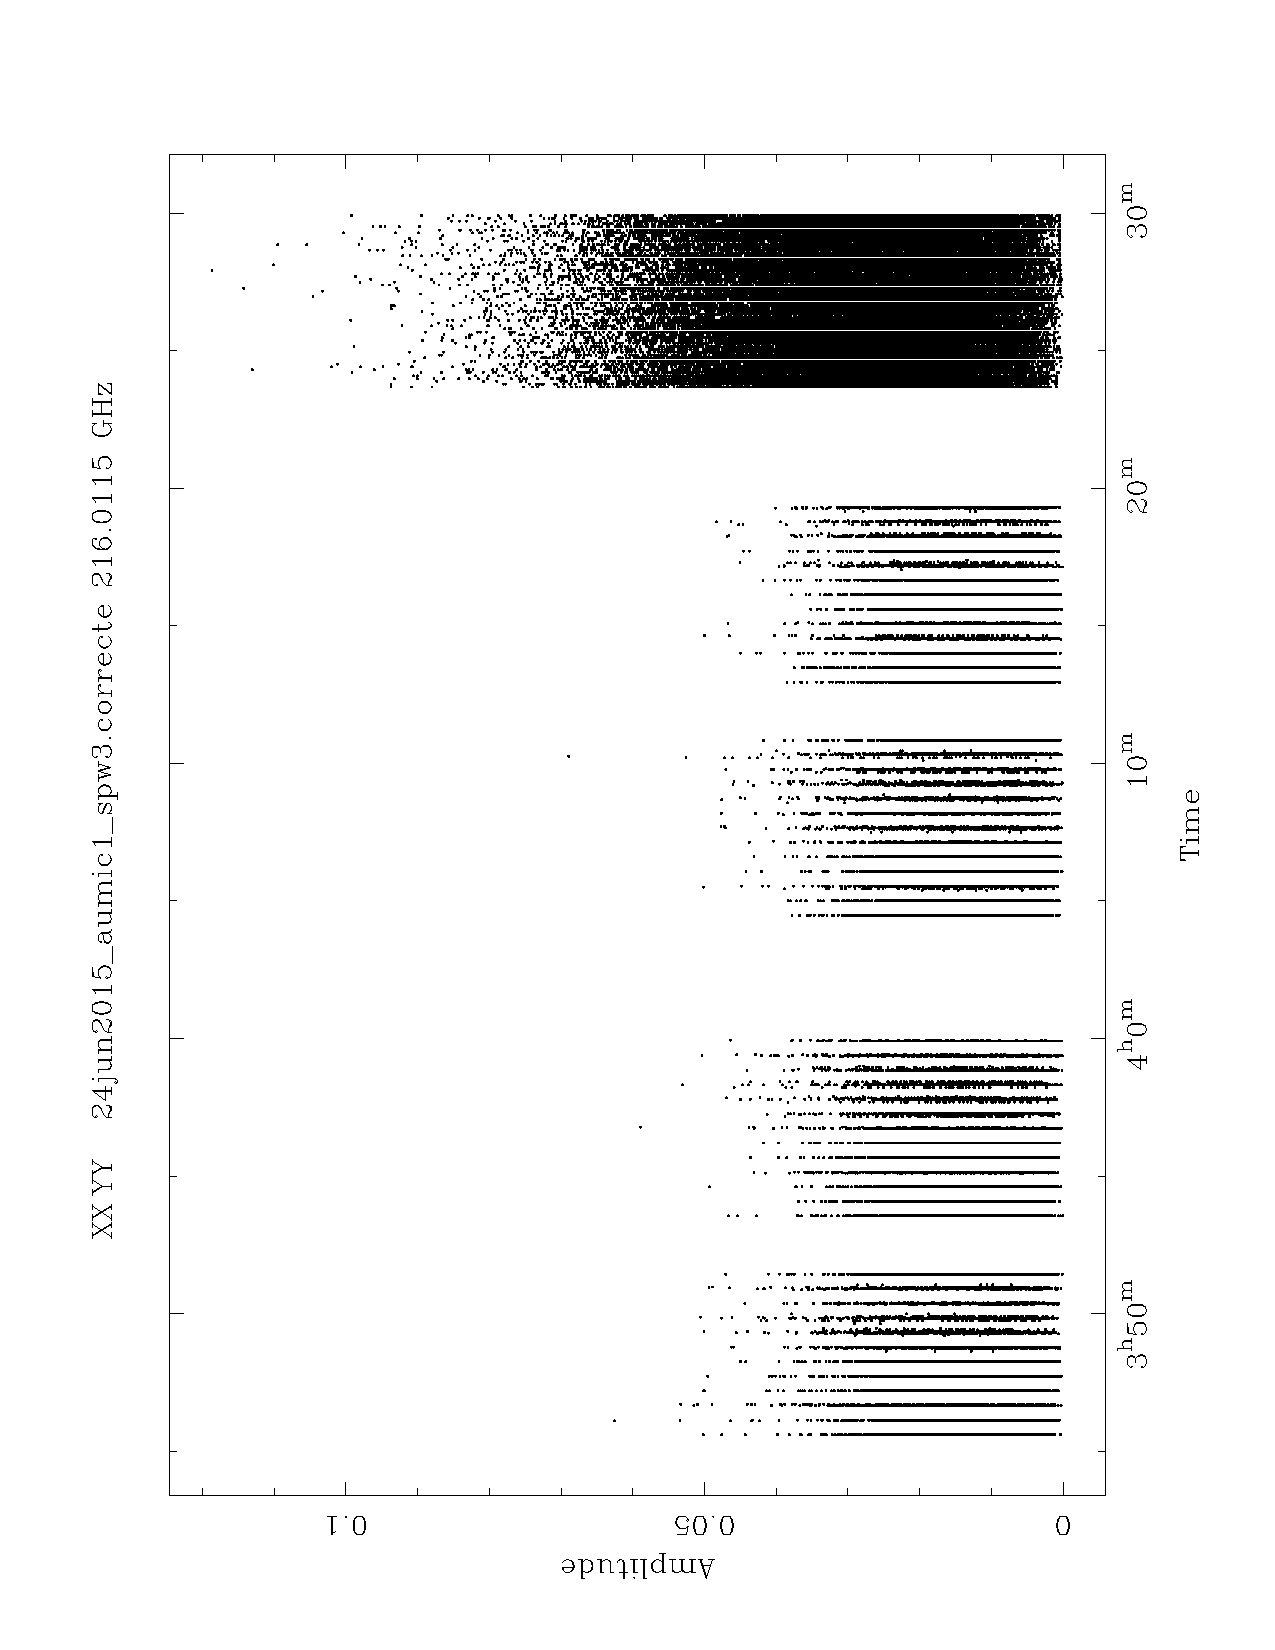
\includegraphics[width=.7\textwidth, angle=-90]{bad_vis_plot}
\end{figure}


\hrulefill
%%%%%%%%%%%%%%%%%%%%%%%%%%%%%%%%%%%%%%%%%%%%%%%%%%%%%%%%

\newday{18 November 2016}

\paragraph{Weights} \ \\
While looking at Kevin's weight correction code, Meredith and I realized that the code only calculates the weights for the \textit{real} component of the visibilities, and does not calculate the imaginary weights. As such, I was applying the real weights to both the real and imaginary visiblities to obtain the $\chi^2$ for my models. This is a decent approximation assuming that the real weights are roughly the same as the imaginary weights, i.e. \textbf{that the real dispersion is roughly the same as the imaginary dispersion}. However, plotting the real weight vs. the imaginary weights implies that this is not the case, and regardless some accuracy is lost using this approximation. Instead, we are calculating the total weight for each point as
\begin{align}
	\label{weight}
	wt_{tot} = \sqrt{wt_{real}wt_{imaginary}}
\end{align}
and inserting the total weights into both the xx and yy polarization columns of each data file.\\
When calculating the corrected weights for each file using the method described above, the code prints the mean absolute difference between the real and imaginary weights, defined as
\begin{align*}
	\mu_{diff} = \frac{\sum |wt_{real}-wt_{imaginary}|}{N}
\end{align*}

The values for $\mu_{diff}$, as well as $\chi^2$s calculated with the corrected weights, are tabulated below.

\begin{tabular}{lrr}
	\toprule
	File                     & Reduced $\chi^2$ & $\mu_{diff}$      \\
	\midrule
	18aug2015\_spw0          & 2.04             & \num{2777.94}     \\
	18aug2015\_spw1          & 2.04             & 3262.7            \\
	18aug2015\_spw2          & 2.04             & 3354.83           \\
	18aug2015\_spw3          & 2.05             & 3136.28           \\
	\textbf{24jun2015\_spw0} & 2.12             & \num{1.04171e+06} \\
	24jun2015\_spw1          & 1.99             & 963318.0          \\
	24jun2015\_spw2          & 2.01             & \num{1.26727e+06} \\
	\textbf{24jun2015\_spw3} & 12.18            & \num{2.39607e+08} \\
	26mar2014\_spw0          & 2.07             & 4755.47           \\
	26mar2014\_spw1          & 2.07             & 5064.5            \\
	26mar2014\_spw2          & 2.06             & 5180.01           \\
	26mar2014\_spw3          & 2.07             & 4431.92           \\
	\bottomrule
\end{tabular}

Using Equation \ref{weight} reduced the reduced $\chi^2$s for the bad spectral windows--this implies that the previously un-included imaginary weights tend to be smaller than the real weights. Kevin's weight correcting code also took about a factor of ten longer to run for the June date than for either of the other two.

\hrulefill
%%%%%%%%%%%%%%%%%%%%%%%%%%%%%%%%%%%%%%%%%%%%%%%%%%%%%%%%
\newday{1 November 2016}

\begin{itemize}
	\item Made sure that Modeling\_Code\_check.py deletes existing .vis files before it remakes them to avoid overwrite failure.
	\item Began setting up check code to do the splitting through miriad, rather than CASA-- hopefully I can use the weights created by Kevin's code for the miriad-split visibilities.
\end{itemize}


\hrulefill
%%%%%%%%%%%%%%%%%%%%%%%%%%%%%%%%%%%%%%%%%%%%%%%%%%%%%%%%
\newday{25 October 2016}

Created a new directory in AU\_Mic titled ``fixing\_spws'' to hold things related to fixing bad spws.\\
\indent Created a specialized version of my modeling code, Modeling\_Code\_check.py, to check $\chi^2$ for different spw splits.

\begin{itemize}
	\item Splitting 24 Jun spws 2 and 3 (one good spw and one bad one) by time to compare $\chi^2$
	\item NOTE: Can just use exportuvfits to split
\end{itemize}


% \hrulefill
%%%%%%%%%%%%%%%%%%%%%%%%%%%%%%%%%%%%%%%%%%%%%%%%%%%%%%%%

% \bibliographystyle{unsrt}
% \bibliography{aumic_notes}

\end{document}
